\section{Description Of The Algorithm}
%Introduce the system model by explaining the FFAST (dual problem - IFFT) architecture and then describe the decoding algorithm - peeling (multiple matches case) and Product code approach (only one exact match case).      
In this section we describe our algorithm, with sample and time complexities that are sub-linear in $N$, to find the locations $\underline{\tau} = (\tau_1, \tau_2, \cdots \tau_L)$ in the string $\xv$, where the string (query) $\yv$ matches. This is achieved by computing the cross-correlation $\rv$ of $\xv$ and $\yv$, defined in Eqn.~\eqref{Eqn:DefCrossCorrelation}, and finding the positions where there is a significant peak. 

The main idea here is that $\RXYv$ is sparse (upto some noise) with dominant peaks at $L$ positions ($\tau$) where the strings match, and noise components at $N-L$ positions where the strings do not match. Consider the case of exact matching,
\begin{equation} \label{eqn:RXY_sparse}
r[m] \ = \left\{
\begin{array}{ll}
  &M , \ \ \  \text{if} \ m \in \mathcal{T} \\
  & n_m , \ \ \ m \in [N]-\mathcal{T}
\end{array} 
\right.  
\end{equation}
where, $ \mathcal{T}:=\{\tau_1, \tau_2, \cdots, \tau_L\}$,
% $M-K \leq v_m \leq M $ is the signal component and
 $n_m$ is the noise component that is induced due to correlation of two i.i.d. sequence of random variables each taking values from $\mathcal{A} := \{+1,-1\}$. The $\rv$ can also be computed as shown below:
\begin{equation}\label{eqn:Rxy_fourier}
  \rv = \underset{\text{ \RNum{1} } } {\mathcal{F}_{N}^{-1}} \ \{ \underset{\text{ \RNum{2} } }{  \mathcal{F}_{N}\{\xv\}}  \odot \ \underset{\text{ \RNum{3} } }{ \mathcal{F}_{N}\{\yv'\}}  \} 
\end{equation} 
where $\mathcal{F}_{N}\{ \cdot \}$ and $\mathcal{F}_{N}^{-1}\{ \cdot \}$ refers to $N$-point discrete Fourier transform and its inverse respectively, $\odot$ is the point-wise multiplication operation and ${ y'[n]} = { y^{*}[-n]}$. Fig.~\ref{fig:notional} presents a notional diagram of our Algorithm.

 As evident from Equation~\ref{eqn:Rxy_fourier}, our algorithm for computing $R_{XY}$ consists of three stages:

\begin{figure}[h!]
	\begin{center}
		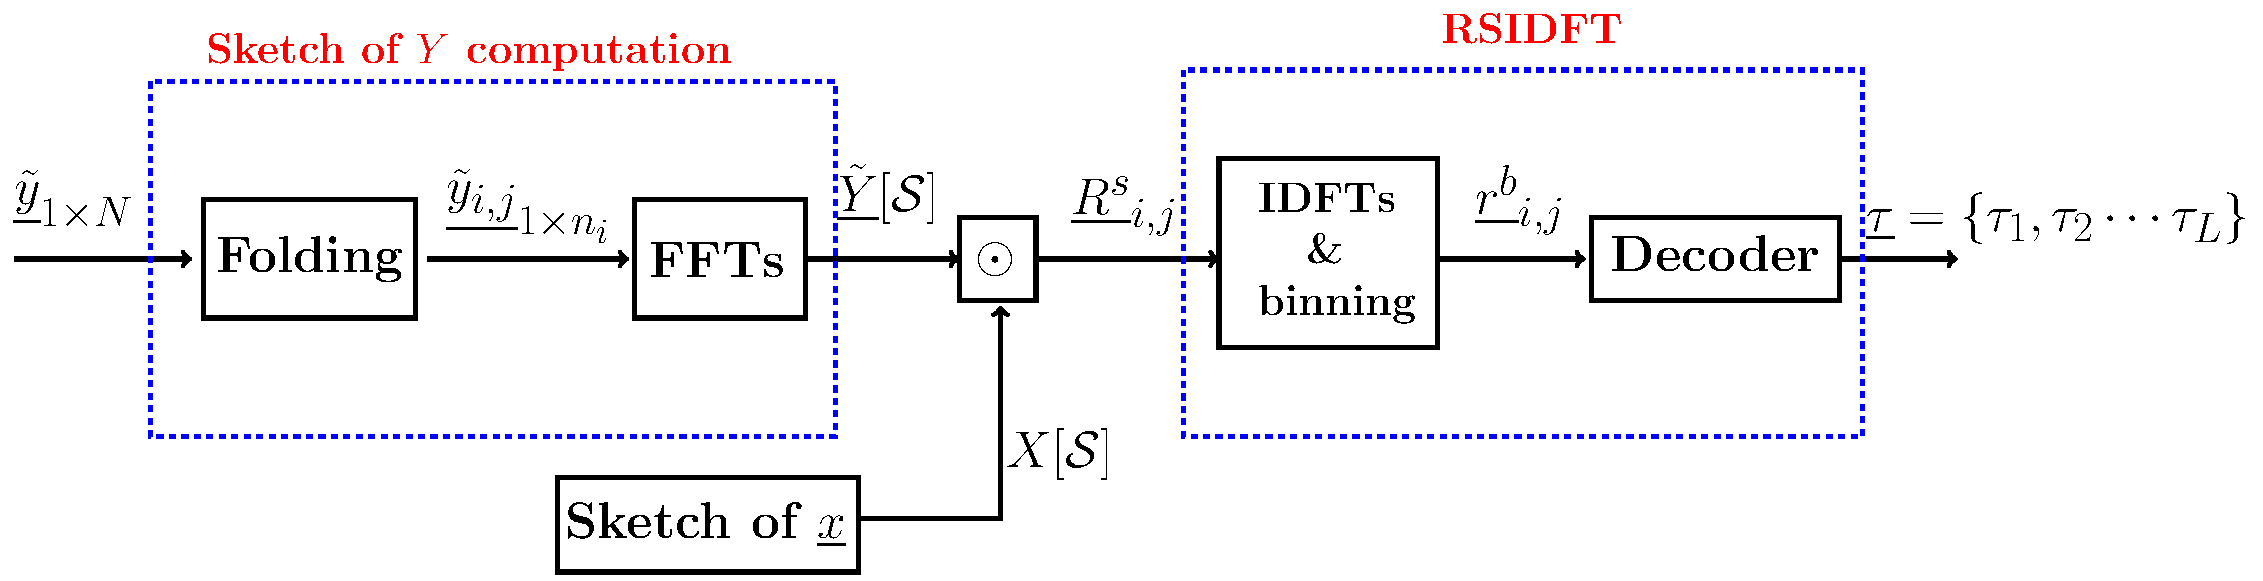
\includegraphics[height=3cm]{Figures/notional_diag} 
	\end{center}	   
	\caption{}\label{fig:notional}
	\vspace{5 pt}
\end{figure}

\begin{enumerate}
\item[\RNum{1}] \textit{Computing sparse $\mathcal{F}^{-1}$}:	

Since $\rv$ is sparse, we use a Robust Sparse Inverse  Discrete Fourier Transform(RSIDFT) framework to compute the $L$-sparse coefficients. The architecture of RSIDFT is similar to FFAST proposed in \cite{pawar2014robust}, but the decoding algorithm has some key modifications to handle the noise model induced in this problem.
 
\subsection{RSIDFT Framework} 	
\label{subsec:RSIDFT}	
	  Let $ \Rv  =  \Xv \odot \Yv'$ be the FFT of the cross-correlation of $\xv$ and $\yv$. We will see in Sec.~\ref{subsec:skteches} how do we compute the required samples of $\Xv$ and $\Yv$ but for this section we will assume that $\Xv$ and $\Yv$ are available and the required samples of $\Rv$ is computed and input to RSIDFT framework. The RSIDFT framework computes the $L$ dominant coefficients of $\rv$ by using only a sub-sampled version of $\Rv$.\\
	  	  
Consider the RSIDFT framework shown in Figure~\ref{fig:rsidft}. The framework consists of {\it $d$-stages} with each stage correpsonding to a sub-sampling factor of $\frac{N}{f_i}$. The design scheme for choosing parameters $\{f_1,f_2,\ldots,f_d\}$ for various regimes of $\mu$ such that $f_i | N$ and $f_i=N^{\alpha}+O(1) \forall i$ are given in \ref{subsec:DesignParameters}. In each stage, there are {\it $B$ branches} with shifts from $\underline{s}\ = [s_1, s_2, \cdots s_B] $, where $s_1 =0$ in the first branch and the rest chosen randomly from $[N^{\alpha}]$. We can also carefully choose the shifts to satisfy mutual coherence property and restricted isometric property described in the analysis section.\\
	   
	 \begin{figure}[h!]
	 	\begin{center}
	 	\resizebox{0.6\textwidth}{!}{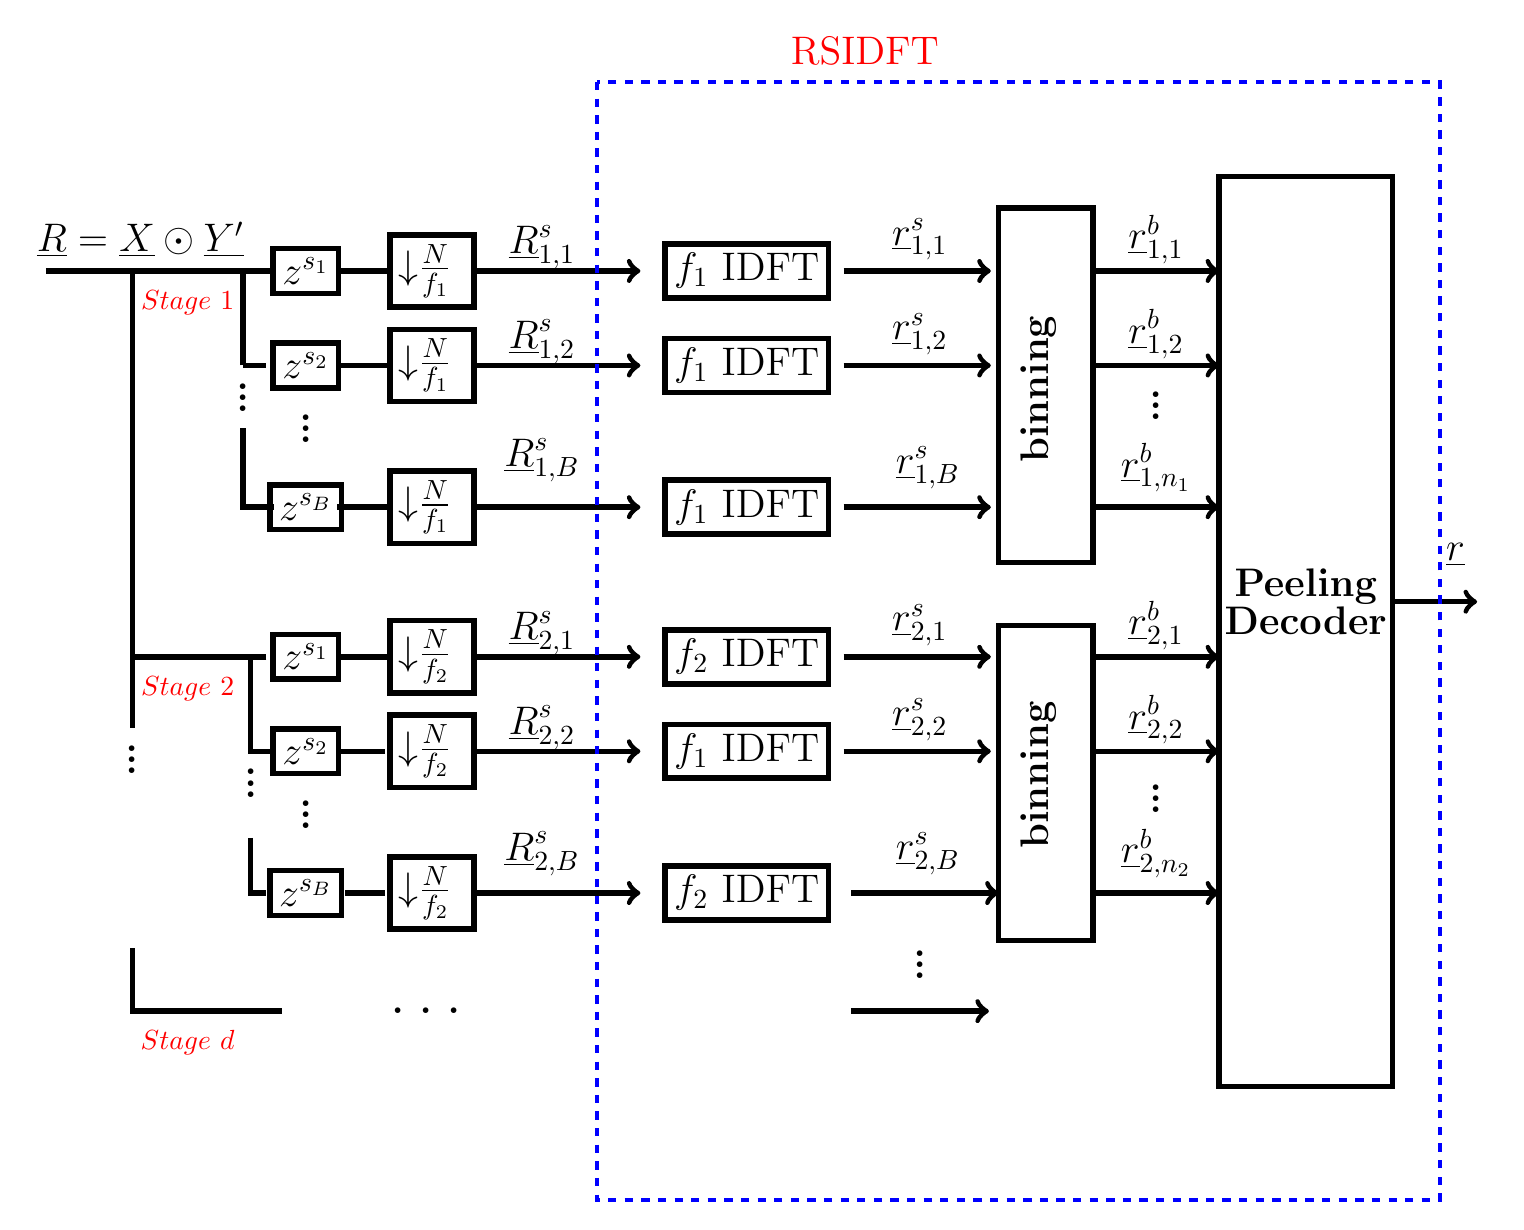
\begin{tikzpicture}

 % Downsampling blocks
\node[draw,align=center,thick,line  width =2pt] at (1.8,4.5) {\Large{$\mathbf{\downarrow} \frac{N}{f_2}$} };
\node[draw,align=center,thick,line  width =2pt] at (1.8,5.7) {\Large{$\mathbf{\downarrow} \frac{N}{f_2}$ }};
\node[draw,align=center,thick,line  width =2pt] (v6) at (1.8,2.7) {\Large{$\mathbf{\downarrow} \frac{N}{f_2}$ }};

\node[draw,align=center,thick,line  width =2pt] at (1.8,9.4) {\Large{$\mathbf{\downarrow} \frac{N}{f_1}$} };
\node[draw,align=center,thick,line  width =2pt] at (1.8,10.6) {\Large{$\mathbf{\downarrow} \frac{N}{f_1}$ }};
\node[draw,align=center,thick,line  width =2pt] at (1.8,7.6) {\Large{$\mathbf{\downarrow} \frac{N}{f_1}$ }};

%  Input lines to the down-sampling block

%  Delay blocks
\node[draw,align=center,thick,line  width =2pt] at (0.2,10.6) {\bf \Large{$z^{s_1}$}};
\node[draw,align=center,thick,line  width =2pt] at (0.2,9.4) {\bf \Large{$z^{s_2}$}};
\node[draw,align=center,thick,line  width =2pt] at (0.2,7.6) {\bf \Large{$z^{s_B}$}};

\node[draw,align=center,thick,line  width =2pt] at (0.2,5.7) {\bf \Large{$z^{s_1}$}};
\node[draw,align=center,thick,line  width =2pt] at (0.2,4.5) {\bf \Large{$z^{s_2}$}};
\node[draw,align=center,thick,line  width =2pt] at (0.2,2.7) {\bf \Large{$z^{s_B}$}};


% paths connecting the delay blocks  
 
 \draw[thick,line  width =2pt] (1.3,9.4) -- (0.6,9.4);
 

\node[line  width =2pt] at (-0.6,9.1) {\Huge{\vdots}};
\node[line  width =2pt] at (0.2,8.7) {\Huge{\vdots}};
\node[line  width =2pt] at (-0.5,4.2) {\Huge{\vdots}};
\node[line  width =2pt] at (0.2,3.8) {\Huge{\vdots}};

 \draw[thick,line  width =2pt] (1.3,10.6) -- (0.6,10.6);
 \draw[thick,line  width =2pt] (-0.6,9.4) -- (-0.6,10.6);
 
% paths connecting the two stages   
 \draw[thick,line  width =2pt] (-0.2,10.6) -- (-2,10.6);
 \draw[thick,line  width =2pt] (-0.6,9.4) -- (-0.3,9.4);
 \draw[thick,line  width =2pt] (-0.3,5.7) -- (-2,5.7);
 \draw[thick,line  width =2pt] (-2,5.7) -- (-2,10.6);
  \draw[thick,line  width =2pt] (-3.1,10.6) -- (-2,10.6);
  \draw[thick,line  width =2pt] (-2,5.7) -- (-2,4.8);
  
  
  % DFT blocks
\node[draw,align=center,thick,line  width =2pt] at (5.8,4.5) {\Large{$f_1$ IDFT}};
\node[draw,align=center,thick,line  width =2pt] at (5.8,5.7) {\Large{$f_2$ IDFT}};
\node[draw,align=center,thick,line  width =2pt] at (5.8,2.7) {\Large{$f_2$ IDFT}};

\node[draw,align=center,thick,line  width =2pt] at (5.8,9.4) {\Large{$f_1$ IDFT}};
\node[draw,align=center,thick,line  width =2pt] at (5.8,10.6) {\Large{$f_1$ IDFT}};
\node[draw,align=center,thick,line  width =2pt] at (5.8,7.6) {\Large{$f_1$ IDFT}};
% Connectors
 \draw[->,thick,line  width =2pt] (2.35,10.6) -- (4.45,10.6);
 \draw[->,thick,line  width =2pt] (2.35,9.4) -- (4.45,9.4);
 \draw[->,thick,line  width =2pt] (2.35,7.6) -- (4.45,7.6);
 
 \draw[->,thick,line  width =2pt] (2.35,5.7) -- (4.45,5.7);
 \draw[->,thick,line  width =2pt] (2.35,4.5) -- (4.45,4.5);
 \draw[->,thick,line  width =2pt] (2.35,2.7) -- (4.45,2.7);

 \draw[->,thick,line  width =2pt] (10.23,10.6) -- (11.8,10.6);
 \draw[->,thick,line  width =2pt] (10.23,9.4) -- (11.8,9.4);
 \draw[->,thick,line  width =2pt] (10.23,7.6) -- (11.8,7.6);
 
 \draw[->,thick,line  width =2pt] (10.23,5.7) -- (11.8,5.7);
 \draw[->,thick,line  width =2pt] (10.23,4.5) -- (11.8,4.5);
 \draw[->,thick,line  width =2pt] (10.23,2.7) -- (11.8,2.7);
 
  \draw[->,thick,line  width =2pt] (7.03,10.6) -- (8.9,10.6);
 \draw[->,thick,line  width =2pt] (7.03,9.4) -- (8.9,9.4);
 \draw[->,thick,line  width =2pt] (7.03,7.6) -- (8.9,7.6);
 
 \draw[->,thick,line  width =2pt] (7.03,5.7) -- (8.9,5.7);
 \draw[->,thick,line  width =2pt] (7.03,4.5) -- (8.9,4.5);
 \draw[->,thick,line  width =2pt] (7.13,2.7) -- (9,2.7);
 
  % Labels
  \node[draw=none,align=center] at (-1.9,11) {\Large{$\underline{R}= \underline{X} \odot \underline{Y'}$}};
  
  \node[draw=none,align=center] at (3.2,10.9) {\Large{$\underline{R}^{s}_{1,1}$}};
  \node[draw=none,align=center] at (3.2,9.7) {\Large{$\underline{R}^{s}_{1,2}$}};
\node[draw=none,align=center] at (3.2,8.2) {\Large{$\underline{R}^{s}_{1,B}$}};

\node[draw=none,align=center] at (3.2,6) {\Large{$\underline{R}^{s}_{2,1}$}};
  \node[draw=none,align=center] at (3.2,4.8) {\Large{$\underline{R}^{s}_{2,2}$}};
  \node[draw=none,align=center] at (3.2,3.2) {\Large{$\underline{R}^{s}_{2,B}$}};

  \node[draw=none,align=center] at (8,11) {\Large{$\underline{r}^{s}_{1,1}$}};
  \node[draw=none,align=center] at (8,9.8) {\Large{$\underline{r}^{s}_{1,2}$}};
  \node[draw=none,align=center] at (8.1,8.1) {\Large{$\underline{r}^{s}_{1,B}$}};
  
    \node[draw=none,align=center] at (11,11) {\Large{$\underline{r}^{b}_{1,1}$}};
  \node[draw=none,align=center] at (11,9.8) {\Large{$\underline{r}^{b}_{1,2}$}};
  \node[draw=none,align=center] at (11,8.1) {\Large{$\underline{r}^{b}_{1,n_1}$}};
  
     \node [draw=none] at (11,9) {\Huge{\vdots}} ;
   
  \node[draw=none,align=center] at (8,6.1) {\Large{$\underline{r}^{s}_{2,1}$}};
  \node[draw=none,align=center] at (8,4.9) {\Large{$\underline{r}^{s}_{2,2}$}};
  \node[draw=none,align=center] at (8.1,3.2) {\Large{$\underline{r}^{s}_{2,B}$}};
  
  \node [draw=none] at (11,4) {\Huge{\vdots}} ;
  
    \node[draw=none,align=center] at (11,6.1) {\Large{$\underline{r}^{b}_{2,1}$}};
  \node[draw=none,align=center] at (11,4.9) {\Large{$\underline{r}^{b}_{2,2}$}};
  \node[draw=none,align=center] at (11,3.2) {\Large{$\underline{r}^{b}_{2,n_2}$}};
  
  \node [draw=none] at (-2,4.5) {\Huge{\vdots}} ;
  
   \node[draw=none,align=center] at (-1.3,10.2) {\color{red}$Stage ~1$};
  \node[draw=none,align=center] at (-1.3,5.3) {\color{red}$Stage ~2$};
   \node[draw=none,align=center] at (-1.3,0.8) {\color{red}$Stage ~d$};
\draw [thick,line  width =2pt](-2,2) -- (-2,1.2) -- (-0.1,1.2) ;
 \node[draw=none,align=center] at (1.8,1.2) {\Huge{\ldots}};
 
\draw [thick,line  width =2pt] (11.8,0.2424) rectangle (14,11.8);
\node (v1) at (7,1.2) {};
\node (v2) at (9,1.2) {};



\node (v11) at (1.3,7.6) {};


\draw  [->,thick,line  width =2pt](v1) edge (v2);
\node at (8,1.9) {\Huge{\vdots}};
\node [text width=3cm, align =center ] at (12.9,6.4) {\Large \bf Peeling \\ Decoder};
\node (v3) at (13.9,6.4) {};
\node (v4) at (15.2,6.4) {};
\draw [thick, ->,line  width =2pt] (v3) edge (v4);
\node at (14.8,7) {\Large{$\underline{r}$}};

\draw[thick,line  width =2pt] (-0.6,8.6) -- (-0.6,7.6) -- (-0.2,7.6);
\draw[thick,line  width =2pt] (0.6,7.6) -- (1.3,7.6);
\draw[thick,line  width =2pt] (-0.5,5.7) -- (-0.5,4.5) -- (-0.2,4.5);
\draw[thick,line  width =2pt] (-0.5,3.4) -- (-0.5,2.7) -- (-0.3,2.7);
\draw [thick,line  width =2pt](0.6,5.7) -- (1.3,5.7);
\draw[thick,line  width =2pt] (0.6,4.5) -- (1.2,4.5);
\draw[thick,line  width =2pt] (0.7,2.7) -- (1.2,2.7);
\draw [dashed, color=blue, line width =1.5pt ] (3.9,13) rectangle (14.6,-1.2);
\node[color =red] at (7.3,13.4) {\Large RSIDFT  };
\draw [thick, line width =2pt]  (9,11.4) rectangle (10.2,6.9);
\draw [thick, line width =2pt]  (9,6.1) rectangle (10.2,2.1);
\node[rotate=90] at (9.5,9.1) {\Large \bf binning};
\node[rotate=90] at (9.5,4.2) {\Large \bf binning};
\end{tikzpicture}}
%	 		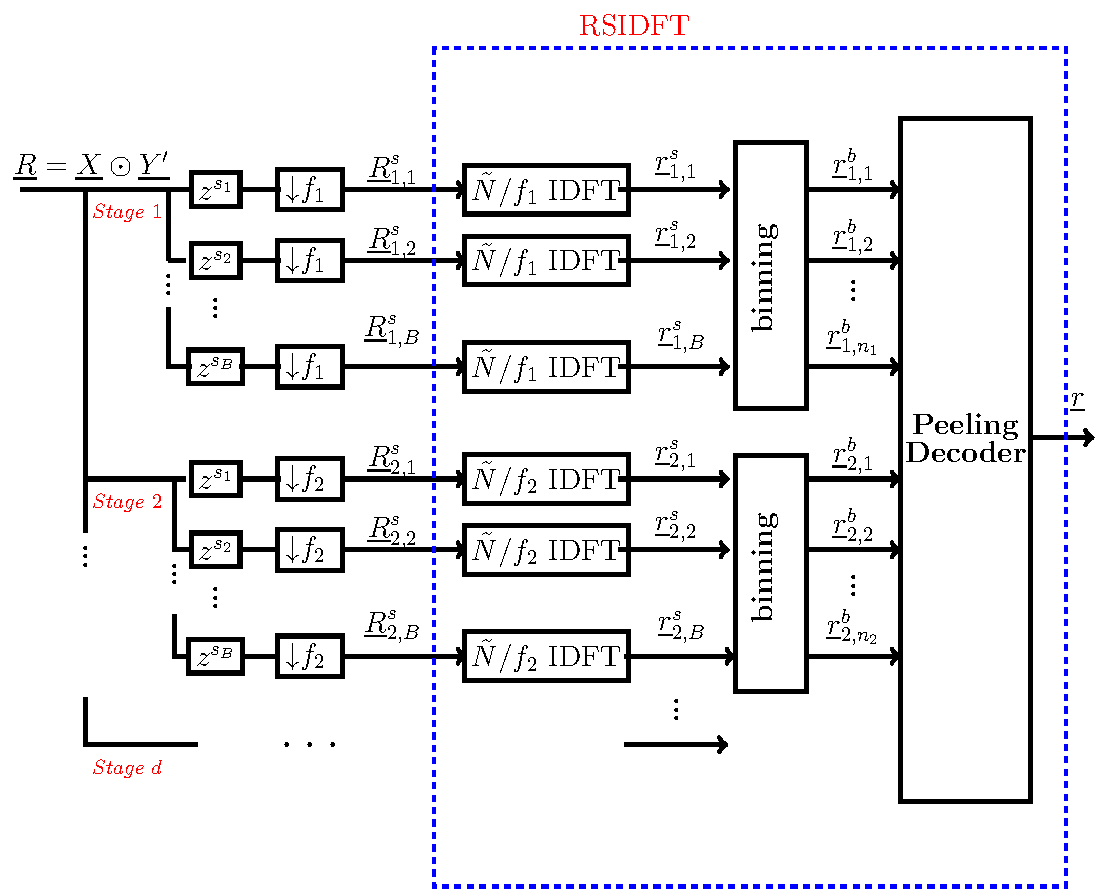
\includegraphics[height=7cm]{Figures/FFAST_Robust} 
	 	\end{center}	   
	 	\caption{ RSIDFT Framework to compute inverse Fourier Transform of a signal $\Rv$ that is sparse in time domain. }\label{fig:rsidft}
	\vspace{5 pt}
	 \end{figure}
	 	
	 Given the input $\Rv$, in branch $j$ of $i^{\text{th}}$ stage or referred to as \textit{branch $(i,j)$} for convenience, RSIDFT sub-samples the signal $\Rv$ at
\begin{align}
\label{Eqn:SamplingSets}
	 \mathcal{S}_{i,j} \coleq \{s_j,\ s_j + n_i,\ s_j + 2n_i,\ \cdots s_j + (f_i-1) n_i\},
\end{align}
where $n_i\coleq \frac{N}{f_i}$ to obtain $\Rv^{s}_{i,j}=\Rv[\mc{S}_{i,j}]$. The sub-sampling operation is followed by a $f_i$-point IDFT in each branch of stage $i$ to obtain $ \rv^{s}_{i,j}$. Notice that $ \rv^{s}_{i,j}$ is an aliased version of $\rv$ due to the property that sub-sampling in Fourier domain is equivalent to aliasing in time domain.\\

	 Let $\rv^{b}_{i,k}$ be the  vector of observations that is formed by combining all $k^{\text{th}}$ coefficients of $\rv^{s}_{i,k}$ (belonging to stage $i$) together as a vector, where $k\in [0:f_i-1]$, i.e.
\[
	  \rv^{b}_{i,k} = \begin{bmatrix}
	 r^{s}_{i,1}[k] \\
	 r^{s}_{i,2}[k] \\
	 \vdots\\
	 r^{s}_{i,B}[k]
	 \end{bmatrix}  
\]
%Let $\mb{W}\coleq[\underline{w}^{0},\underline{w}^{1},\ldots, \underline{w}^{N-1}]$. where $•\underline{w}^{k}=[e^{j2\pi ks_1},e^{j2\pi ks_2},\ldots, e^{j2\pi ks_{B}}]$. Then
More formally we can write the relationship between the the observation vectors $\rv^b_{i,j}$ at bin $(i,j)$ and sparse vector to be estimated $\rv$ as:
\begin{align}
	\label{Eqn:Generator Equation}
	\rv^b_{i,k}= \mb{W}_{i,k} \times
	\begin{bmatrix}
		r[k+(0)f_i] \\
		r[k+(1)f_i] \\
		\vdots\\
		r[k+(n_i-1)f_i]
	\end{bmatrix}
\end{align}

where we refer to $\mb{W}_{i,k}$ as the sensing matrix at bin $(i,k)$ and can be defined as  
\begin{align}\label{Eqn:Sensing Matrix}
	\mb{W}_{i,k} = \left[\underline{w}^{k},\underline{w}^{k+f_i},\ldots, \underline{w}^{k+(n_i-1)f_i}\right] \text{and} ~\underline{w}^{k}=
	\begin{bmatrix}
		e^{\frac{j2\pi ks_1}{N}}\\
		e^{\frac{j2\pi ks_2}{N}}\\
		\vdots\\
		e^{\frac{j2\pi ks_B}{N}}
	\end{bmatrix}
\end{align}

\begin{figure}[h!]
	\begin{center}
		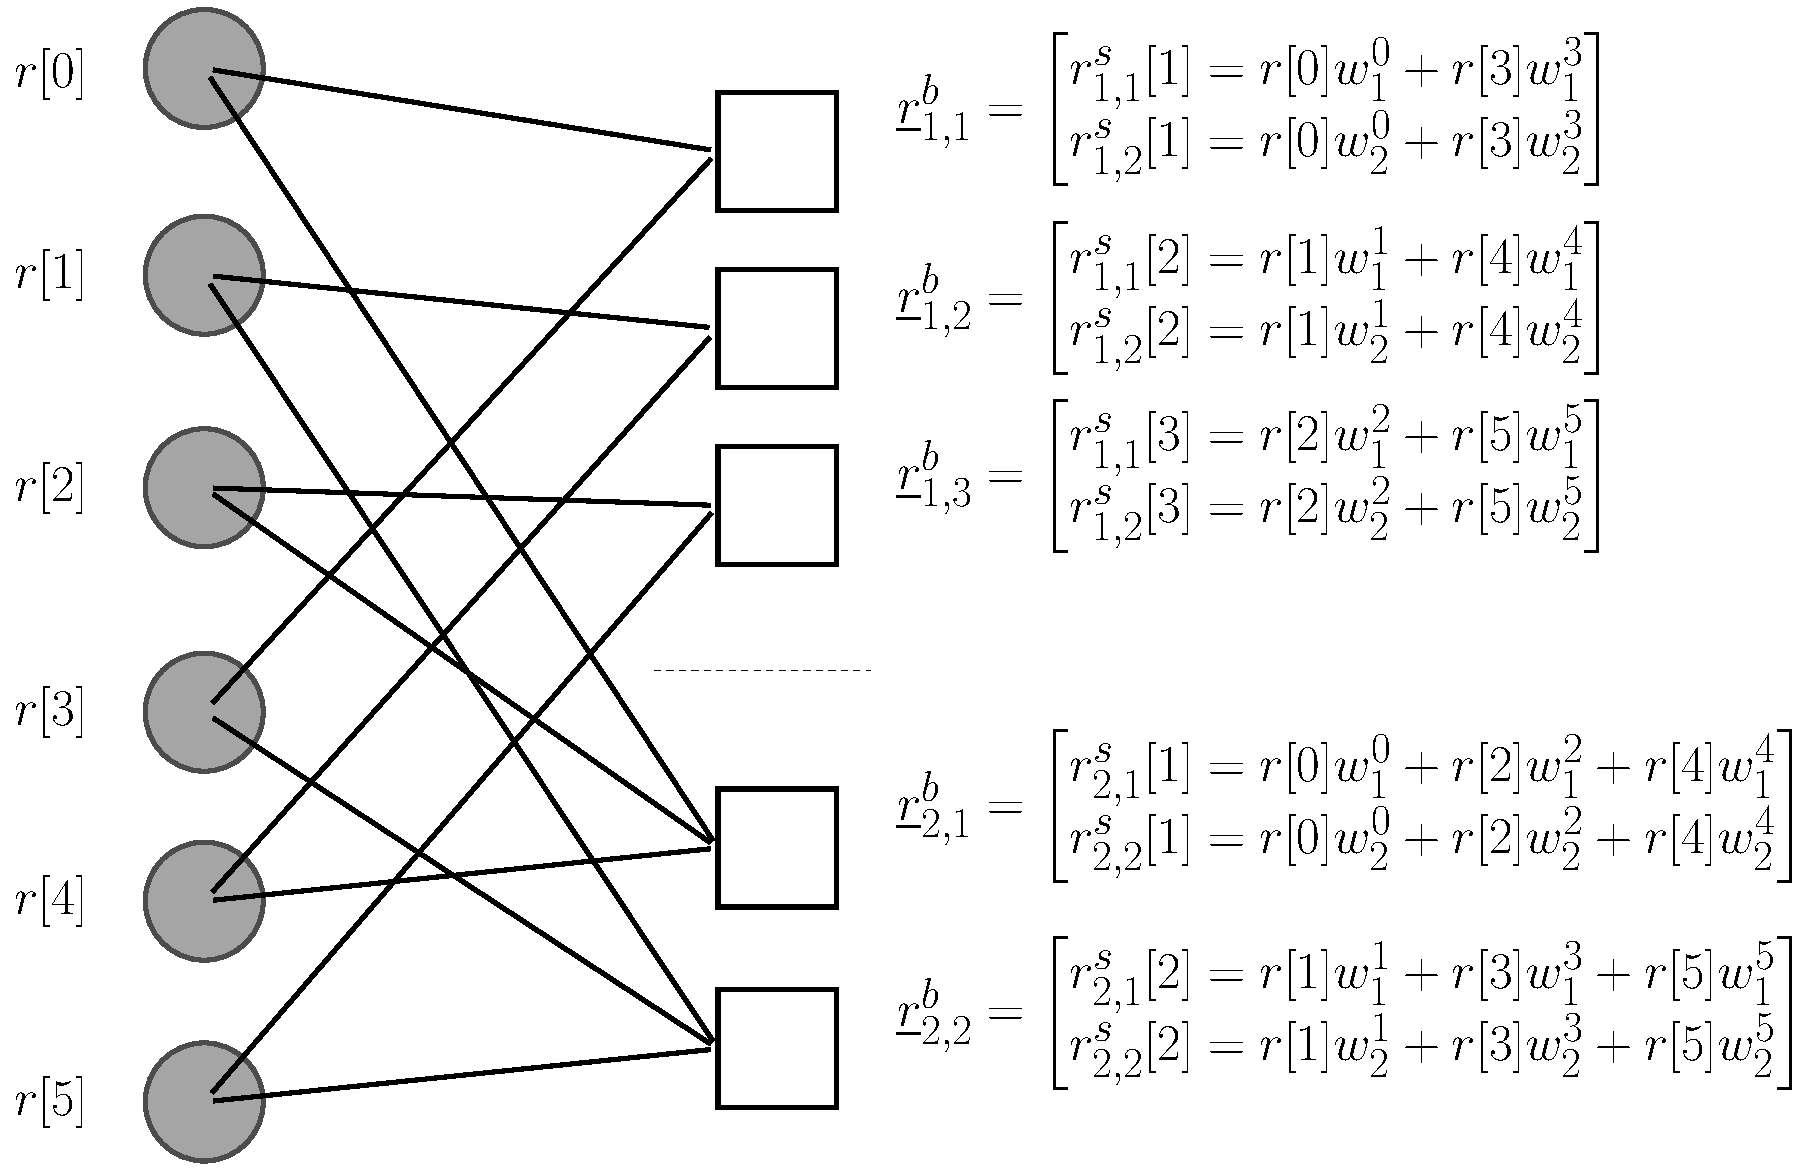
\includegraphics[height=7cm]{Figures/Factorgraph} 
	\end{center}	   
	\caption{Example of a Tanner graph formed in a RSIDFT framework with system parameters being $d=2$, $B=2$, $N=6$, $f_1 = 2$ and $f_2=3$. The variable nodes (colored gray circles) represent the cross-correlation vector $\rv$ and the bin nodes (uncolored white boxes) represent the binned observation vector $\rv_{i,k}^b$. The figure also illustrates the relationship between $\rv_{i,k}^b$ and $\rv$.}\label{fig:factorgraph}
	\vspace{5 pt}
\end{figure}

In Fig.~\ref{fig:factorgraph} we represent the relation between $\rv$ and $\tilde{\rv}^{b}\coleq[\rv^{b}_{1,1},\rv^{b}_{1,2},\ldots,\rv^{b}_{1,n_1},\ldots, \rv^{b}_{2,1},\ldots,\rv^{b}_{2,n_2},\ldots, \rv^{b}_{B,1},\ldots,\rv^{b}_{B,n_B}]$
%, aliased versions of the cross-correlation vector $\rv$ concatenated together
via an example using Tanner graph. We refer to $\tilde{\rv}^{b}$ as sensing signal. The nodes on the left, which we refer to as {\it variable nodes}, represent the $N$ elements of vector $\rv$. And similarly the nodes on the right, which we refer to as {\it bin nodes}, represent the $\sum_{i\leq B} n_i$ sub-sensing signals. We will now describe the decoding algorithm which takes the sensing signal $\tilde{\rv}^b$ as input and estimates the $L$-sparse $\rv$.	 

\subsection{Decoder}		
	%\textcolor[rgb]{0,0.3,0.7}{Maybe remove Each coefficient of $\rv^{b}_{i,p_i}$ is a bin that has $N^{\alpha}$ coefficients from $\RXYv$ hashed into it. This can be seen using a Tanner graph with $\RXYv$ as the left nodes (bit nodes) and the aliased coefficients $\rv^{b}_{i,p_i}$ as the right nodes (check-nodes).}
	
	Observe from the Tanner graph that the degree of each bit node is $d$ and that of each bin node is approximately $N^{\alpha}$. 
We refer to a bin node as {\it zero-ton} (or $\msc{H}_z$) if the number of variable nodes with significant amplitude connected to the bin node is zero. The {\it singleton ($\msc{H}_s$), double-ton ($\msc{H}_d$) and multi-ton ($\msc{H}_m$)} bin nodes are defined similarly where the number of significant variable nodes connected are one, two and greater than two, respectively. The peeling decoder has the following three steps in the decoding process.\\

%\begin{itemize}
%\itemsep4pt
%\item \textbf{Bin Classification}:
\subsubsection{Bin Classification} In this step a bin node is classified as a zero-ton or a singleton or a multi-ton. At bin $(i,j)$ the classification is done based on  comparing the first observation $r^{b}_{i,j}[1]$, which corresponds to zero shift, with a predefined threshold. Let the value of $r^{b}_{i,j}[1]$ be $z$, then the classification rules can be written as follows:\\
%{\it Exact Matching:} 
%\begin{align}
%\label{Eqn:BinClassifExact}
%\widehat{\msc{H}}_{i,j}=
%\begin{cases}
%\msc{H}_z &  		z/M < 0.5 \\
%\msc{H}_s &	 0.5 \leq z/M \leq 1.5 \\ 
%\msc{H}_d \text{ or } \msc{H}_m  &       z/M > 1.5
%\end{cases}
%\end{align}
%\textit{Approximate Matching}: 
\begin{align}
\label{Eqn:BinClassifApprox}
\widehat{\msc{H}}_{i,j}=
\begin{cases}
\msc{H}_z &  	 z/M < \gamma_1\\
\msc{H}_s &	  \gamma_1 < z/M < \gamma_2  \\
\msc{H}_d  &    \gamma_2  < z/M <  \gamma_3\\ 
\msc{H}_m &      z/M > \gamma_3\\
\end{cases}
\end{align}
where $(\gamma_1,\gamma_2,\gamma_3)=(\frac{1-2\eta}{2},\frac{3-4\eta}{2},\frac{5-6\eta}{2})$. Note that for the case of exact matching $\eta=0$.
			   
%\item \textbf{Singleton decoding}:
\subsubsection{Singleton decoding}
 If a bin node $(i,j)$ is classified as a singleton, we need to identify the position of the significant non-zero variable node connected to it. This is done by correlating the observation vector $\rv^{b}_{i,j}$ with each column of  $\mb{W}_{i,j} \coleq [\underline{w}^{j},\underline{w}^{j+n_i},\ldots,   \underline{w}^{j+(f_i-1)n_i}]$ and choose the index that maximizes the correlation value.
\begin{align*}
 \hat{k} = \underset{k\in\{j+l n_i\}}{\argmax}\  \underline{w}^{k} ~ \rv^{b}_{i,j}
\end{align*}
 The value of the variable node connected to  the singleton bin  is estimated as follows:\\
% \textit{Exact Matching}: 
% $$\hat{r}[\hat{k}]=M\\
% $$
% \textit{Approximate Matching}: 
 $$
 \hat{r}[\hat{k}]=M(1-\eta).
 $$
 Note that for the case of exact matching we know the value to be exactly equal to $M$ which is our estimate in the case of exact matching ($\eta=0)$. But in the case of approximate matching the actual value of $x[k]\in\{M(1-2\eta),\ldots,M-1,M\}$ and our estimate $ \hat{r}[\hat{k}]=M(1-\eta)$, the mid-point of the range, is only a loose approximate, this would suffice for our purposes as we are mainly interested in recovering only the positions of matches i.e. the indices of the sparse coefficients in $\rv$ nit their values. \\
 %If a bin $(i,j)$ is classified as singleton, we denote the singleton decoder output of bin $(i,j)$ as $(\hat{k},\hat{r}[\hat{k}])=${\it SINGLETON-DEC}$(i,j)$.\\ % $\msc{H}_{i,j}$.% as $\msc{H}_s(\hat{k},\hat{r}[\hat{k}])$.\\
			 

%\item \textit{Peeling Process: }
\subsubsection{Peeling Process} The main idea behind the peeling based decoder is to find a singleton bin, identify the significant variable node connected to the bin, decode it's value and remove it's contribution from all the bin nodes connected to that variable node. Although the main idea is similar for exact matching and the approximate matching scenarios, there are some subtle differences in their implementation.\\

{\it Exact Matching}: In the case of exact matching, we remove the decoded variable node's contribution from all the bin nodes it is connected to.\\
{\it Approximate Matching}: In this case we remove the decoded variable node's contribution only from singleton and double-ton bins and do not alter the bins which are classified to be multi-tons with degree more than two.\\

We present the overall recovery algorithm, which comprises of {\it bin classification, singleton decoding} and {\it peeling process}, in the Algorithm \ref{Algo:decoder} pseudo-code.

\def\gap{4pt}
\begin{algorithm}[h!]
\caption{Peeling based recovery algorithm}
\label{Algo:decoder}
\begin{algorithmic}
\State Compute $\widehat{\msc{H}}_{i,j}$ for $i\in[B], j\in[n_i]$. See Eqn. \eqref{Eqn:BinClassifApprox}
%\eqref{Eqn:BinClassifExact} \&
\vspace{\gap}
\While {$\exists~ i,j:\widehat{\msc{H}}_{i,j}= \msc{H}_s$,}
\vspace{\gap}
  \State $(\hat{k},\hat{r}[\hat{k}])=${\bf Singleton-Decoder}$(\rv^b_{i,j})$
\vspace{\gap}
  \State Assign $\hat{r}[\hat{k}]$ to $\hat{k}^{\text{th}}$ variable in bin $(i,j)$
\vspace{\gap}
  \For{$(i_0,j_0)\in\msc{N}(\hat{k})$}
\vspace{\gap}
	   \State $\rv^{b}_{i_0,j_0}\gets\rv^{b}_{i_0,j_0}-\hat{r}[\hat{k}]\mb{g}_{\hat{k}}$   \hspace{45.5ex} {\it Exact Matching}
	   \vspace{\gap}
	   \State $\rv^{b}_{i_0,j_0}\gets\rv^{b}_{i_0,j_0}-\hat{r}[\hat{k}]\mb{g}_{\hat{k}}$   \hspace{10ex} only if $\widehat{\msc{H}}_{i_0,j_0}=\msc{H}_s$ or $\msc{H}_d$ \hspace{10ex} {\it Approximate Matching}
	   \vspace{\gap}
	   \State Recompute $\widehat{\msc{H}}_{i_0,j_0}$
      \EndFor
\EndWhile
\end{algorithmic}
\end{algorithm}

\begin{algorithm}[h!]
\caption{Singleton-Decoder}
\label{Algo:SingletonDecoder}
\begin{algorithmic}
\State{\bf Input:} $\rv^b_{i,j}$
\vspace{\gap}
\State{\bf Output:} $(\hat{k},\hat{r}[\hat{k}])$
\vspace{\gap}
\State Estimate singleton index to be $ \hat{k} = \underset{k\in\{j+l n_i\}}{\argmax}\  \underline{w}^{k} ~ \rv^{b}_{i,j}$
\vspace{\gap}
  \State Estimate the value to be:$$ \hat{r}[\hat{k}]=
   \begin{cases}
   M & \text{ Exact Matching case}\\
  M-\frac{K}{2} & \text{ Approximate Matching case}
  \end{cases}
  $$
%  \vspace{\gap}
%  \State\hspace{23ex}           $\hat{r}[\hat{k}]=$ \hspace{10ex} Approximate Matching case
\end{algorithmic}
\end{algorithm}

\subsubsection{Choosing $\alpha$ and $f_i$ for various $\mu$}
\label{subsec:DesignParameters}
For a given value of $\mu$, we will describe how to choose the parameters $d$ and $f_i$.\\
{\it Exact Matching}: Find $d\in \mbb{Z}_+$ such that $\mu\in(\frac{1}{d},\frac{1}{d-1})\cup(1-\frac{1}{d-1},1-\frac{1}{d})$\\
{\it Approximate Matching}: If $\mu\in(\frac{1}{8},\frac{7}{8})$, choose $d=8$. Else find $d\in\mathbb{Z}_+$ such that $\mu\in(\frac{1}{d},\frac{1}{d-1})\cup(1-\frac{1}{d-1},1-\frac{1}{d})$ and $d\geq 8$ \\

\begin{itemize}
\item Find a factorization for signal length $N=\prod_{i=0}^{d-1} \mcl{P}_i$ such that the set of integers $\{\mcl{P}_0,\mcl{P}_1,\ldots,\mcl{P}_{d-1}\}$ are pairwise co-prime and all the $\mcl{P}_i$ are approximately equal
\item More precisely, let $\mcl{P}_i=\mathbf{F}+O(1) ~\forall i$ and choose $f_i=N/\mcl{P}_i$
\item Our choice of design parameters results in $f_i\approx N^{\alpha}$ where $\alpha=1-\frac{1}{d}$.
\end{itemize} 


To summarize our choice of design parameters, both in the exact and approximate matching cases, for any $0<\mu<1$, we choose the down-sampling factors $f_i$ to be approximately equal to $N^{\alpha}$ in all the $d$-stages where $\alpha$ satisfies:
\begin{equation}
\label{Eqn:IneqMuAlpha}
\alpha>\max(\mu,1-\mu)
\end{equation}
which is easy to verify.

\subsection{Sketches of $\Xv$ and $\Yv$} 
\label{subsec:skteches}		 
 As we have already seen in Sec.~\ref{subsec:RSIDFT} the RSDIFT framework requires the values of $\Rv(=\Xv\odot \Yv)$ only at indices $\mc{S}$ or in other words we need $\Xv$ and $\Yv$ only at the indices $\mc{S}$. \\
 %We exploit this property of sparsity to compute $\RXYv$ by using only a subset of samples from $\Xv = \mathcal{F}\{\xv\} $ and $\Yv' = \mathcal{F}\{\yv'\} $, each sampled at positions $l \in \mathcal{S}$, where $\mathcal{S} = \mathcal{S}_{1,1} \cup \mathcal{S}_{1,2} \cup \cdots \cup \mathcal{S}_{i,j} \cup  \mathcal{S}_{d,B} \subset \{ 0,1,\cdots ,N-1 \}$ and $\mathcal{S}_{i,j}$, $1 \leq i \leq d $ and  $1 \leq j \leq B $ are disjoint sets of size $|\mathcal{S}_{i,j}| \approxeq N^{1-\alpha}$ with periodic sample points from $[N]$ given by 
% 
% \begin{equation}
% \label{eqn:sampling_sets}\mathcal{S}_{i,j} = \{s_j,\ s_j + f_i,\ s_j + 2f_i,\ \cdots s_j + \lfloor{\frac{N}{f_i} }\rfloor f_i \}
% \end{equation}
%   where $s_j$'s and $f_i$'s are constants chosen based on the requirements from Robust Sparse Inverse Fourier Transform (RSIDFT) framework described in Section~\ref{subsec:RSIDFT}.

%\item[\RNum{1}] 
\textit{Computing the sketch of $\xv$}: We assume that the sketch of $\xv$, $ \Xv[\mc{S}]= \{X[i],i\in \mc{S}\}$ is pre-computed and stored in a database.  \\

\textit{Computing the sketch of $\yv$}: For every new query $\yv$, only $\{\Yv'[\mc{S}_{i,j}],i\in[d],j\in[B]\}$ needs to be computed where the subsets $\mc{S}_{i,j}$ are defined in Eq. \eqref{Eqn:SamplingSets}. Naively, the FFT algorithm can be used to compute $\Yv'$ and the required subset of coefficients can be taken but this would be of $O(N \log N)$ complexity. We observe that $\Yv'[\mc{S}_{i,j}]$ is $\Yv'$ shifted by $s_j$ and sub-sampled by a factor of $f_i$. Thus for a given $(i,j)$ this corresponds to, in time domain, a point-wise multiplication by $[1,W_{s_j},W_{s_j}^2,\ldots,W_{s_j}^{N-1}]$ followed by \textit{folding} the signal into $f_i$ number of length $\frac{N}{f_i}$ signals and adding them up resulting in a single length $\frac{N}{f_i}$ signal denoted by $\yv'_{i,j}$. Formally the \textit{folding} operation can be described as follows:
	  \begin{equation}
	  	\yv'_{i,j} = \sum \limits_{m = 0}^{f_i-1} \yv'[mn_i:(m+1)n_i-1] \odot [W_{s_j}^{mn_i},W_{s_j}^{mn_i+1},\ldots, W_{s_j}^{(m+1)n_i-1}],\qquad W_{s_j}=e^{\frac{j2\pi s_j}{N}}
%	  		  	\yv'_{i,j}[p] = \sum \limits_{m = 0}^{f_i} \y'[p + mn_i] e^{j \frac{2 \pi s_j}{N} } 
	  \end{equation}
	  where $n_i=\frac{N}{f_i}$. Taking $n_i$-point DFT of $\yv'_{i,j}$ produces $\Yv'[\mc{S}_{i,j}]$ i.e. $\Yv'$ sampled only at $\mathcal{S}_{i,j}$ indices which is what we need in branch $(i,j)$. To obtain all the samples in $\mathcal{S}$ required for the RSDIFT framework, the \textit{folding} technique needs to be carried out for each $(i,j)$, for $i\in[d],j\in[B]$, a total of $\approx dB~~ N^{1-\alpha}$-point DFTs.
\end{enumerate}


%The idea behind this folding technique is to induce aliasing in $\yv'$ and then taking a smaller point Fourier Transform to compute the sub-sampled version $\Yv'$. Aliasing is induced by folding the signal $\yv'$ into blocks of length $N^{1-\alpha}$ and adding them. The desired sub-sampling patterns in frequency domain are induced by multiplying $\yv'$ with suitable exponentials. Let us denote the aliased versions of $\yv'$ by $\yv_{i,j}'$. Then, $\yv_{i,j}'$ is given by